\section{5. Inequalities}\label{inequalities}

\subsection{5.1 Markov and Chebyshev
Inequalities}\label{markov-and-chebyshev-inequalities}

\textbf{Theorem 5.1 (Markov's Inequality)}. Let \(X\) be a non-negative
random variable and suppose that \(\mathbb{E}(X)\) exists. For any
\(t > 0\),

\[ \mathbb{P}(X > t) \leq \frac{\mathbb{E}(X)}{t} \]

\textbf{Proof}.

\[ 
\mathbb{E}(X)
=\int_0^\infty xf(x) dx
=\int_0^t xf(x) dx + \int_t^\infty xf(x) dx
\geq \int_t^\infty xf(x) dx
\geq t \int_t^\infty f(x) dx
= t \mathbb{P}(X > t)
\]

\textbf{Theorem 5.2 (Chebyshev's Inequality)}. Let
\(\mu = \mathbb{E}(X)\) and \(\sigma^2 = \mathbb{V}(X)\). Then,

\[ \mathbb{P}(|X - \mu| \geq t) \leq \frac{\sigma^2}{t^2} 
\quad \text{and} \quad
\mathbb{P}(|Z| \geq k) \leq \frac{1}{k^2} \]

where \(Z = (X - \mu) / \sigma\). In particular,
\(\mathbb{P}(|Z| > 2) \leq 1/4\) and \(\mathbb{P}(|Z| > 3) \leq 1/9\).

\textbf{Proof}. We use Markov's inequality to conclude that

\[ \mathbb{P}(|X - \mu| \geq t) = \mathbb{P}(|X - \mu|^2 \geq t^2) \leq \frac{\mathbb{E}(X - \mu)^2}{t^2} = \frac{\sigma^2}{t^2} \]

The second part follows by setting \(t = k \sigma\).

\subsection{5.2 Hoeffding's Inequality}\label{hoeffdings-inequality}

Hoeffding's inequality is similar in spirit to Markov's inequality but
it is a sharper inequality. We present the result here in two parts. The
proofs are in the technical appendix.

\textbf{Theorem 5.4}. Let \(Y_1, \dots, Y_n\) be independent
observations such that \(\mathbb{E}(Y_i) = 0\) and
\(a_i \leq Y_i \leq b_i\). Let \(\epsilon > 0\). Then, for any
\(t > 0\),

\[ \mathbb{P}\left( \sum_{i=1}^n Y_i \geq \epsilon \right) \leq e^{-t\epsilon} \prod_{i=1}^n e^{t^2(b_i - a_i)^2 / 8} \]

\textbf{Theorem 5.5}. Let \(X_1, \dots, X_n \sim \text{Bernoulli}(p)\).
Then, for any \(\epsilon > 0\),

\[ \mathbb{P}(|\overline{X}_n - p| > \epsilon) \leq 2e^{-2n\epsilon^2} \]

Hoeffding's inequality gives us a simple way go create a
\textbf{confidence interval} for a binomial parameter \(p\). We will
discuss confidence intervals later but here is the basic idea. Let
\(\alpha > 0\) and let

\[ \epsilon_n = \left\{ \frac{1}{2n} \log \left( \frac{2}{\alpha} \right) \right\}^{1/2} \]

By Hoeffding's inequality,

\[ \mathbb{P}(|\overline{X}_n - p| > \epsilon_n) \leq 2e^{-2n\epsilon_n^2} = \alpha \]

Let \(C = (\overline{X}_n - \epsilon, \overline{X}_n + \epsilon)\).
Then,
\(\mathbb{P}(\text{not } C \in p) = \mathbb{P}(|\overline{X}_n - p| > \epsilon) \leq \alpha\).
Hence, \(\mathbb{P}(p \in C) \geq 1 - \alpha\), that is, the random
interval \(C\) traps the true parameter \(p\) with probability
\(1 - \alpha\); we call \(C\) a \(1 - \alpha\) confidence interval. More
on this later.

\subsection{5.3 Cauchy-Schwartz and Jensen
Inequalities}\label{cauchy-schwartz-and-jensen-inequalities}

This section contains two inequalities on expected values that are often
useful.

\textbf{Theorem 5.7 (Cauchy-Schwartz Inequalities)}. If \(X\) and \(Y\)
have finite variances then

\[ \mathbb{E}|XY| \leq \sqrt{\mathbb{E}\left(X^2\right) \mathbb{E}\left(Y^2\right)} \]

Recall that a function \(g\) is \textbf{convex} if for each \(x, y\) and
each \(\alpha \in [0, 1]\),

\[ g(\alpha x + (1 - \alpha)y) \leq \alpha g(x) + (1 - \alpha) g(y) \]

If \(g\) is twice differentiable, then the convexity reduces to checking
that \(g''(x) \geq 0\) for all \(x\). It can be shown that if \(g\) is
convex then it lies above any line that touches \(g\) at some point,
called a tangent line. A function \(g\) is \textbf{concave} if \(-g\) is
convex. Examples of convex functions are \(g(x) = -x^2\) and
\(g(x) = \log x\).

\textbf{Theorem 5.8 (Jensen's Inequality)}. If \(g\) is convex then

\[ \mathbb{E}g(X) \geq g(\mathbb{E}X) \]

If \(g\) is concave then

\[ \mathbb{E}g(X) \leq g(\mathbb{E}X) \]

\textbf{Proof}. Let \(L(x) = a + bx\) be a line, tangent to the \(g(x)\)
at the point \(\mathbb{E}(X)\). Since \(g\) is convex, it lies above the
line \(L(x)\). So,

\[ \mathbb{E}g(X) \geq \mathbb{E}L(X) = \mathbb{E}(a + bX) = a + b\mathbb{E}(X) = L(\mathbb{E}(X)) = g(\mathbb{E}(X))\]

From Jensen's inequality we see that
\(\mathbb{E}X^2 \geq (\mathbb{E}X)^2\) and
\(\mathbb{E}(1/X) \geq 1 / \mathbb{E}(X)\). Since log is concave,
\(\mathbb{E}(\log X) \leq \log \mathbb{E}(X)\). For example, suppose
that \(X \sim N(3, 1)\). Then \(\mathbb{E}(1 / X) \geq 1/3\).

\subsection{5.4 Technical Appendix: Proof of Hoeffding's
Inequality}\label{technical-appendix-proof-of-hoeffdings-inequality}

We will make use of the exact form of Taylor's theorem: if \(g\) is a
smooth function, then there is a number \(\xi \in (0, u)\) such that
\(g(u) = g(0) + u g'(0) + \frac{u^2}{2}g''(\xi)\).

\textbf{Proof of Theorem 5.4}. For any \(t > 0\), we have, from Markov's
inequality, that

\[ \mathbb{P}\left( \sum_{i=1}^n Y_i \geq \epsilon \right) = \mathbb{P}\left( t \sum_{i=1}^n Y_i \geq t \epsilon \right)
= \mathbb{P}\left( e^{t \sum_{i=1}^n Y_i} \geq e^{t \epsilon} \right) \leq e^{-t\epsilon} \mathbb{E}\left( e^{t \sum_{i=1}^n Y_i}\right) = e^{-t\epsilon} \prod_i \mathbb{E}\left(e^{tY_i}\right) \]

Since \(a_i \leq Y_i \leq b_i\), we can write \(Y_i\) as a convex
combination of \(a_i\) and \(b_i\), namely,
\(Y_i = \alpha b_i + (1 - \alpha) a_i\) where
\(\alpha = (Y_i - a_i) / (b_i - a_i)\). So, by the convexity of
\(e^{ty}\) we have

\[ e^{tY_i} \leq \frac{Y_i - a_i}{b_i - a_i} e^{tb_i} + \frac{b_i - Y_i}{b_i - a_i} e^{ta_i} \]

Take expectations of both sides and use the fact that
\(\mathbb{E}(Y_i) = 0\) to get

\[ \mathbb{E}e^{tY_i} \leq - \frac{a_i}{b_i - a_i} e^{tb_i} + \frac{b_i}{b_i - a_i} e^{ta_i} = e^{g(u)} \]

where \(u = t(b_i - a_i)\),
\(g(u) = -\gamma u + \log (1 - \gamma + \gamma e^u)\) and
\(\gamma = -a_i / (b_i - a_i)\).

Note that \(g(0) = g'(0) = 0\). Also, \(g''(u) \leq 1/4\) for all
\(u > 0\). By Taylor's theorem, there is a \(\xi \in (0, u)\) such that

\[ g(u) = g(0) + u g'(0) + \frac{u^2}{2} g(\xi) = \frac{u^2}{2} g(\xi) \leq \frac{u^2}{8} = \frac{t^2(b_i - a_i)^2}{8} \]

Hence,

\[ \mathbb{E}e^{tY_i} \leq e^{g(u)} \leq e^{t^2(b_i - a_i)^2/8} \]

and the result follows.

\textbf{Proof of Theorem 5.5}. Let \(Y_i = (1 / n)(X_i - p)\). Then
\(\mathbb{E}(Y_i) = 0\) and \(a \leq Y_i \leq b\) where \(a = -p/n\) and
\(b = (1 - p) / n\). Also, \((b - a)^2 = 1/n^2\). Applying Theorem 5.4
we get

\[ \mathbb{P}\left(\overline{X}_n - p > \epsilon\right) = \mathbb{P}\left( \sum_i Y_i > \epsilon \right) \leq e^{-t\epsilon} e^{t^2/(8n)}\]

The above holds for any \(t > 0\). In particular, take
\(t = 4n\epsilon\) and we get
\(\mathbb{P}\left(\overline{X}_n - p > \epsilon\right)  \leq e^{-2n\epsilon^2}\).
By a similar argument we can show that
\(\mathbb{P}\left(\overline{X}_n - p < \epsilon\right)  \leq e^{-2n\epsilon^2}\).
Putting those together we get
\(\mathbb{P}\left(|\overline{X}_n - p| >  \epsilon\right)  \leq 2e^{-2n\epsilon^2}\).

\subsection{5.6 Exercises}\label{exercises}

\textbf{Exercise 5.6.1}. Let \(X \sim \text{Exponential}(\beta)\). Find
\(\mathbb{P}(|X - \mu_X| > k \sigma_X)\) for \(k > 1\). Compare this to
the bound you get from Chebyshev's inequality.

\textbf{Solution}.

Let \(F\) be the CDF of \(X\). We have:

\begin{align}
\mathbb{P}(|X - \mu_X| > k \sigma_X) &= 1 - \mathbb{P}(-k \sigma_X < X - \mu_X < k \sigma_X) \\
&= 1 - \mathbb{P}(\mu_X - k \sigma_X < X < \mu_X + k \sigma_X) \\
&= 1 - F(\mu_X + k \sigma_X) + F(\mu_X - k \sigma_X) \\
&= 1 - 1 + \exp\left\{ -\frac{\left(\beta + k \beta\right)^+}{\beta} \right\} + 1 - \exp\left\{-\frac{\left(\beta - k \beta\right)^+}{\beta} \right\} \\
&= 1 + e^{-(1+k)^+ } - e^{-(1-k)^+} 
\end{align}

where \((a)^+ = \max \{ a, 0 \}\).

On the other hand, Chebyshev's bound provides, for \(t = k\sigma_X\),

\[ \mathbb{P}(|X - \mu_X| \geq k \sigma_X) \leq \frac{\sigma_X^2}{k^2 \sigma_X^2}  = \frac{1}{k^2} \]

which is a weaker bound.

\begin{python}
import numpy as np
import matplotlib.pyplot as plt

def f(k):
    return 1 + np.exp(-np.maximum(1+k, 0)) - np.exp(-np.maximum(1 - k, 0))

def chebyshev(k):
    # Limit upper bound to 1, since probability is always under 1
    return np.minimum(1 / (k**2), 1)

kk = np.arange(0.01, 10, step = 0.01)

plt.figure(figsize=(12, 8))

plt.plot(kk, f(kk), label='Calculated probability')
plt.plot(kk, chebyshev(kk), label='min(Chebyshev bound, 1)')
plt.yscale('log')
plt.xlabel('k')
plt.ylabel('Probability bound')
plt.legend(loc='lower left')
plt.show()
\end{python}

\begin{figure}[H]
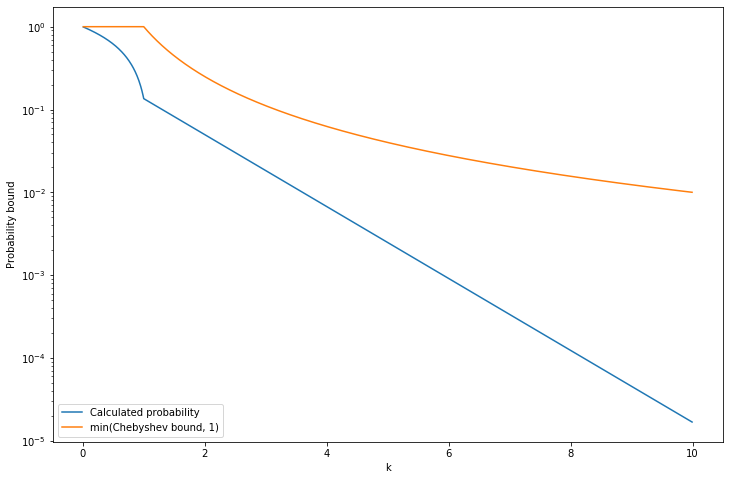
\includegraphics[width=0.9\linewidth,height=0.2\textheight,keepaspectratio]{Figure-05-01}
\end{figure}

\textbf{Exercise 5.6.2}. Let \(X \sim \text{Poisson}(\lambda)\). Use
Chebyshev's inequality to show that
\(\mathbb{P}(X \geq 2\lambda) \leq 1 / \lambda\).

\textbf{Solution}. We have \(\mu_X = \lambda\) and
\(\sigma_X^2 = \lambda\), so Chebyshev's gives us:

\[ \mathbb{P}(|X - \lambda| \geq t) \leq \frac{\lambda}{t^2} \]

If we make \(t = \lambda\), we get

\[ \mathbb{P}(X \geq 2\lambda) = \mathbb{P}(|X - \lambda| \geq \lambda) \leq \frac{1}{\lambda} \]

\textbf{Exercise 5.6.3}. Let
\(X_1, \dots, X_n \sim \text{Bernoulli}(p)\) and
\(\overline{X}_n = n^{-1} \sum_{i=1}^n X_i\). Bound
\(\mathbb{P}(|\overline{X}_n - p| > \epsilon)\) using Chebyshev's
inequality and using Hoeffding's inequality.

Show that, when \(n\) is large, the bound from Hoeffding's inequality is
smaller than the bound from Chebyshev's inequality.

\textbf{Solution}. Note that \(\mathbb{E}(\overline{X}_n) = p\) and
\(\mathbb{V}(\overline{X}_n) = p(1-p) / n\), since
\(n \overline{X}_n \sim \text{Binomial}(n, p)\).

Using Chebyshev's inequality,

\[ \mathbb{P}(|\overline{X}_n - p| \geq \epsilon) \leq \frac{p(1 - p)}{n \epsilon^2} \]

Using Hoeffding's inequality,

\[ \mathbb{P}(|\overline{X}_n - p| > \epsilon) \leq 2e^{-2n\epsilon^2} \]

The bound provided by Hoeffding's inequality is
\(O(e^{-2n\epsilon^2})\), while the bound provided by Chebyshev's
inequality is \(O(n^{-1})\), therefore the bound from Hoeffding's
inequality is smaller for a sufficiently large \(n\).

\textbf{Exercise 5.6.4}. Let
\(X_1, \dots, X_n \sim \text{Bernoulli}(p)\).

\textbf{(a)} Let \(\alpha > 0\) be fixed and define

\[ \epsilon_n = \sqrt{\frac{1}{2n} \log \left( \frac{2}{\alpha}\right)} \]

Let \(\hat{p}_n = n^{-1} \sum_{i=1}^n X_i\). Define
\(C_n = (\hat{p}_n - \epsilon_n, \hat{p}_n + \epsilon_n)\). Use
Hoeffding's inequality to show that

\[ \mathbb{P}(p \in C_n) \geq 1 - \alpha \]

We call \(C_n\) a \emph{\(1 - \alpha\) confidence interval for \(p\)}.
In practice, we truncate the interval so it does not go below 0 or above
1.

\textbf{(b) (Computer Experiment)} Let's examine the properties of this
confidence interval. Let \(\alpha = 0.05\) and \(p = 0.4\). Conduct a
simulation study to see how often the interval contains \(p\) (called
the coverage). Do this for various values of \(n\) between 1 and 10000.
Plot the coverage versus \(n\).

\textbf{(c)} Plot the length of the interval versus \(n\). Suppose we
want the length of the interval to be no more than .05. How large should
\(n\) be?

\textbf{Solution}.

\textbf{(a)} The result is immediate from replacing \(\epsilon_n\) into
Hoeffding's inequality,

\[ \mathbb{P}(|\hat{p}_n - p| > \epsilon_n) \leq 2e^{-2n\epsilon_n^2} = \alpha \]

since \(\mathbb{E}(\hat{p}_n) = p\).

\textbf{(b)}

\begin{python}
import numpy as np
from scipy.stats import bernoulli
from tqdm import tqdm_notebook

alpha = 0.05
p = 0.4

B = 50000
N = 10000

nn = np.arange(1, N + 1)
epsilon_n = np.sqrt((1 / (2 * nn)) * np.log(2 / alpha))

p_hat = np.empty((B, N))
for i in tqdm_notebook(range(B)):
    X = bernoulli.rvs(p, size=N, random_state=i)
    p_hat[i] = np.cumsum(X) / nn

coverage = np.mean((p_hat + epsilon_n >= p) & (p_hat - epsilon_n <= p), axis=0)
\end{python}

\begin{python}
import matplotlib.pyplot as plt

plt.figure(figsize=(12, 8))
plt.plot(nn, coverage)
plt.xlabel('n')
plt.ylabel('Coverage')
plt.show()
\end{python}

\begin{figure}[H]
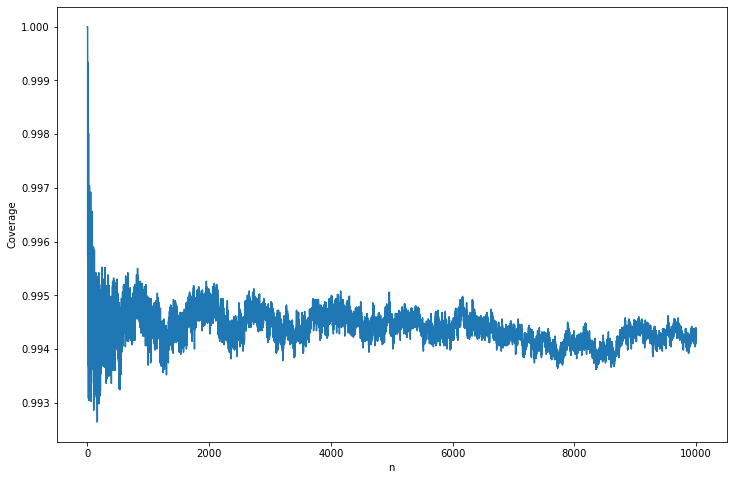
\includegraphics[width=0.9\linewidth,height=0.2\textheight,keepaspectratio]{Figure-05-02}
\end{figure}

\textbf{(c)} The length of the interval is
\(\min \{\hat{p}_n + \epsilon_n, 1 \} - \max \{ \hat{p}_n - \epsilon_n, 0\}\).
As \(\hat{p}_n \rightarrow p\), let's plot the approximation on the
limit case, which is just \(2 \epsilon_n\).

\begin{python}
plt.figure(figsize=(12, 8))
plt.plot(nn, 2 * epsilon_n, label='Interval length')
plt.xlabel('n')
plt.ylabel(r'$2\epsilon_n$')
plt.hlines(.05, xmin=0, xmax=N, color='red', label='Threshold')
plt.yscale('log')
plt.legend(loc='upper right')
plt.show()

selected_n = nn[np.argmax(2 * epsilon_n <= .05)]
print('Smallest n with interval length under .05: %i' % selected_n)
\end{python}

\begin{figure}[H]
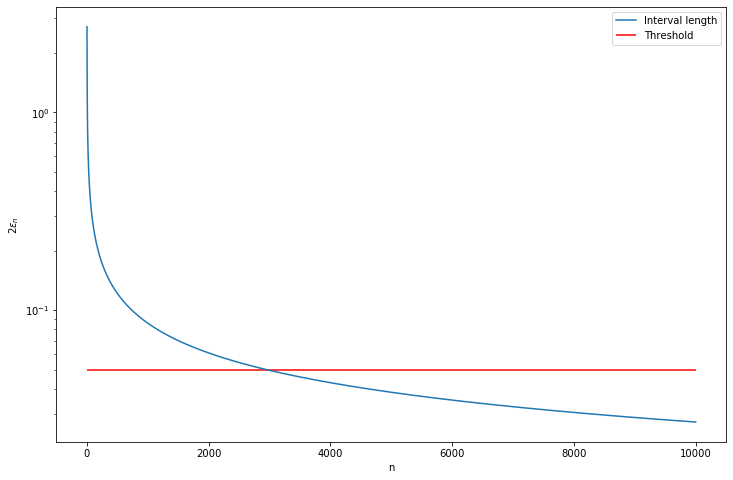
\includegraphics[width=0.9\linewidth,height=0.2\textheight,keepaspectratio]{Figure-05-03}
\end{figure}

\begin{console}
Smallest n with interval length under .05: 2952
\end{console}
